\documentclass[conference]{IEEEtran}
\IEEEoverridecommandlockouts
\usepackage{cite}
\usepackage{amsmath,amssymb,amsfonts}
\usepackage{graphicx}
\usepackage{xcolor}
\usepackage{booktabs}
\usepackage{hyperref}
\hypersetup{hidelinks}
\usepackage{multirow}
\usepackage{tikz}
\usetikzlibrary{shapes,arrows,positioning,fit,backgrounds,calc,shadows}
\usepackage{subcaption}
\setlength{\textfloatsep}{7pt plus 1pt minus 2pt}
\setlength{\floatsep}{6pt plus 1pt minus 2pt}
\setlength{\dbltextfloatsep}{7pt plus 1pt minus 2pt}
\setlength{\dblfloatsep}{6pt plus 1pt minus 2pt}

\begin{document}

\title{Dual-Innovation Neural-Kalman Fusion for Causal Indoor Localization}

\author{
\IEEEauthorblockN{Utkarsh Agrawal\textsuperscript{*}\IEEEauthorrefmark{1},
Jayendra Vijay Birhade\textsuperscript{*}\IEEEauthorrefmark{1},
Neel Kanth Kundu\IEEEauthorrefmark{2}}
\IEEEauthorblockA{\IEEEauthorrefmark{1}Department of Computer Science and Engineering,
Indian Institute of Technology Delhi, New Delhi, India}
\IEEEauthorblockA{\IEEEauthorrefmark{2}Centre for Applied Research in Electronics,
Indian Institute of Technology Delhi, New Delhi, India\\
Email: neelkanth@iitd.ac.in}
\thanks{\textsuperscript{*}These authors contributed equally to this work.}
}

\maketitle

\begin{abstract}
Indoor localization can combine Wi-Fi, magnetic, and inertial sensing, but practical fusion requires a causal mechanism for reconciling sparse spatial measurements with drifting pedestrian dead reckoning (PDR) when measurement availability and reliability vary over time. We propose a decoupled learned state-space estimator in which a Wi-Fi heatmap multilayer perceptron (MLP) and an 84-frame gravity-referenced magnetic convolutional neural network (CNN) independently produce Cartesian position measurements, while PDR supplies relative motion. DualKalmanNet forms separate Wi-Fi and magnetic innovations and uses a gated recurrent unit (GRU) to predict separate $2\times2$ correction gains. Availability masks remove missing modalities, and a training-normalized magnetic log-uncertainty score scales the magnetic correction. After freezing the model and evaluation protocol, temporal fusion is evaluated once on 60 untouched survey-graph-constrained trajectories within a fixed surveyed environment. With 1~Hz Wi-Fi, the weighted model reduces mean error from 0.523~m for Wi-Fi-only KalmanNet to 0.490~m, a 6.4\% reduction. Under degraded Wi-Fi (5~s updates with 40\% access-point dropout), it reduces mean error from 1.734~m to 0.900~m (48.1\%) and lowers pointwise P90 error from 3.767~m to 1.845~m.
\end{abstract}

\begin{IEEEkeywords}
Indoor positioning, KalmanNet, learned state-space estimation, sensor fusion, pedestrian dead reckoning, Wi-Fi fingerprinting, magnetic localization.
\end{IEEEkeywords}

\section{Introduction}

Indoor localization supports location-based services, smart buildings, and emergency navigation, where satellite-based positioning is often unreliable indoors~\cite{radar}. Wi-Fi fingerprinting provides infrastructure-based absolute position estimates~\cite{horus}, pedestrian dead reckoning (PDR) provides high-rate relative motion but accumulates drift~\cite{nnwifipdr}, and indoor magnetic structure provides an additional spatial fingerprint~\cite{overviewdatasets}. These modalities have already been combined in prior systems: Li \emph{et al.} integrate PDR, Wi-Fi fingerprinting, and magnetic matching~\cite{li2016hybrid}; Bolat and Akcakoca combine Wi-Fi, magnetic field, and inertial navigation~\cite{hybridwifi}; and DeepPositioning learns joint Wi-Fi--magnetic localization~\cite{deeppos}. Thus, combining the three sensing sources is not itself our contribution. The problem addressed here is how to apply spatial corrections from asynchronous learned measurements to a drifting motion state when measurement availability and reliability change over time.

For fusion step $t\geq 1$, PDR produces the prior state $\mathbf{x}_{t}^{-}=\mathbf{x}_{t-1}+\mathbf{u}_{t}$. A spatial measurement $\mathbf{z}_{j,t}$ from modality $j\in\{\mathrm{wifi},\mathrm{mag}\}$ produces the innovation $\mathbf{y}_{j,t}=\mathbf{z}_{j,t}-\mathbf{x}_{t}^{-}$. Fusion therefore requires deciding how strongly each correction $\mathbf{K}_{j,t}\mathbf{y}_{j,t}$ should modify the prior. Prior work addresses parts of this problem using adaptive factor-graph weighting for Wi-Fi/PDR~\cite{wang2020factorgraph}, neural Wi-Fi/PDR fusion~\cite{nnwifipdr}, and learned Kalman-style state estimation~\cite{kalmannet}. The distinction sought here is architectural rather than an initialization fix: two learned spatial measurements are represented in one Cartesian state space and influence the causal state update through separate, history-dependent gain matrices.

Learned spatial models provide complementary measurement functions. DeepPositioning combines Wi-Fi and magnetic fingerprints using deep learning~\cite{deeppos}; MINLOC applies a CNN to magnetic field patterns~\cite{minloc}; and Zardkoohi \emph{et al.} use bidirectional long short-term memory for magnetic sequence localization~\cite{bilstmmag}. Because a bidirectional recurrent estimator uses both past and future sequence context, it is not directly suitable for streaming causal inference without reformulation. Our objective is not to attribute prior limitations to initialization, but to separate spatial measurement extraction from temporal correction and make each available measurement explicit in the state update.

In this work, we propose a decoupled causal learned state-space architecture for multimodal indoor localization, where \emph{multimodal} denotes heterogeneous Wi-Fi, magnetic, and inertial measurements. First, a Wi-Fi heatmap MLP and a gravity-referenced magnetic CNN independently produce Cartesian position measurements; the magnetic CNN also provides a scalar relative uncertainty score. Second, DualKalmanNet forms separate Cartesian innovations and predicts separate $2\times2$ Wi-Fi and magnetic gain matrices, while availability masks remove unavailable modalities. Third, a training-normalized magnetic confidence weight explicitly attenuates uncertain magnetic corrections. The temporal fusion experiment evaluates independent survey-graph-constrained trajectories within one surveyed environment. The architecture can be reused after site-specific surveying and training, but the present fusion results do not constitute building-agnostic or plug-and-play unseen-device validation.

Section \ref{sec:measurements} defines measurements and preprocessing; Section \ref{sec:architecture} presents the estimator; Section \ref{sec:setup} gives training and evaluation; Section \ref{sec:results} reports results; and Section \ref{sec:conclusion} concludes the paper.

\section{Sensor Measurements and Preprocessing}\label{sec:measurements}

Assume a targeted indoor environment with $N$ identifiable Wi-Fi access points (APs) and a Cartesian reference grid containing $M$ spatial cells. We use $n$ for raw inertial/magnetic samples and $t$ for the lower-rate fusion steps. The phone-side quantities are a sparse Wi-Fi received signal strength indicator (RSSI) vector $\mathbf{s}_t\in\mathbb{R}^N$, a magnetometer vector $\mathbf{m}_n\in\mathbb{R}^3$, an accelerometer vector $\mathbf{a}_n\in\mathbb{R}^3$, and a causal heading observation $\hat{\theta}_n$. The estimator state is $\mathbf{x}_t=[x_t,y_t]^T\in\mathbb{R}^2$. Availability indicators $m_{\mathrm{wifi},t},m_{\mathrm{mag},t}\in\{0,1\}$ specify whether a new Wi-Fi or magnetic measurement is available at fusion step $t$.

\paragraph{Wi-Fi preprocessing.}
The raw Wi-Fi scan $\mathbf{s}_t \in \mathbb{R}^N$ is preprocessed into $\tilde{\mathbf{s}}_t \in [0,1]^N$. Undetected APs are stored at the $-100$~dBm floor; clipping and affine rescaling then give
\begin{equation}
\tilde{s}_{t,i}=\frac{\operatorname{clip}(s_{t,i},-90,-30)+90}{60},
\label{eq:wifi_norm}
\end{equation}
so an undetected AP maps to zero without a separate branch.

For database construction, the static magnetic survey coordinate is used as the common 2-D map frame. A Wi-Fi scan is attached to a magnetic visit only when mode, scenario, phone, user, and timestamped filename match exactly; basename-only matches are not used. The Wi-Fi file's recorded coordinate is retained as audit metadata but is not silently substituted for the magnetic survey coordinate. Visits without a unique exact Wi-Fi match remain magnetic-only records.

\paragraph{Magnetic preprocessing.}
The magnetic path begins with gravity-referenced survey preprocessing. For raw sample $n$, the implementation uses the instantaneous normalized acceleration
\begin{equation}
\hat{\mathbf{a}}_n=\frac{\mathbf{a}_n}{\|\mathbf{a}_n\|}
\label{eq:mag_gravity_proxy}
\end{equation}
as a gravity-direction proxy and computes
\begin{align}
m_{N,n} &= \|\mathbf{m}_n\|,
& m_{V,n} &= \mathbf{m}_n^T\hat{\mathbf{a}}_n,
\nonumber\\
m_{H,n} &= \sqrt{\max(m_{N,n}^2-m_{V,n}^2,0)},
\nonumber\\
\delta_n &= \operatorname{atan2}(m_{V,n},m_{H,n}).
\label{eq:mag_features}
\end{align}
We collect these channels in
\begin{equation}
\mathbf{f}^{\mathrm{mag}}_n=
\begin{bmatrix}m_{N,n}&m_{V,n}&m_{H,n}&\delta_n\end{bmatrix}^{T}
\in\mathbb{R}^{4}.
\label{eq:mag_feature_vector}
\end{equation}
These quantities are invariant to a common rigid rotation of the phone when $\hat{\mathbf{a}}_n$ is a valid gravity proxy. The processed survey database stores the mean and standard deviation of each quantity over a static visit. The magnetic-map trainer subtracts each phone's mean feature value, averages the centered visit means at each surveyed node, and interpolates the four channels onto the same 1~m Cartesian environment grid used by the Wi-Fi model.

The per-phone centering defines a survey-specific magnetic feature domain. The present fusion evaluation operates inside this centered domain. Because no causal alignment procedure is implemented for an uncalibrated handset, the magnetic fusion results are scoped to the surveyed, device-normalized domain rather than unseen-phone magnetic deployment.

\paragraph{Inertial inputs.}
For PDR, the accelerometer stream is reduced to $a_n=\|\mathbf{a}_n\|$. The heading observation $\hat{\theta}_n$ is treated as a causal external input rather than as a quantity inferred from future trajectory information. The synthetic evaluation generates this observation from the latent path plus the noise process in Section~\ref{sec:setup}; a deployable raw-sensor heading estimator is outside the scope of the current experiment.

\section{Proposed State-Space Estimator}\label{sec:architecture}

The estimator combines two absolute spatial measurements with relative PDR motion. The Wi-Fi branch supplies intermittent Cartesian anchors, the magnetic branch supplies a causal sequence-based position measurement and relative uncertainty score, and PDR propagates motion between absolute updates. DualKalmanNet then converts these signals into a single causal state correction. Figure~\ref{fig:arch_diagram} shows the functional signal flow of one fusion update; the component models are detailed below.

\begin{figure*}[t]
\centering
\resizebox{0.96\textwidth}{!}{
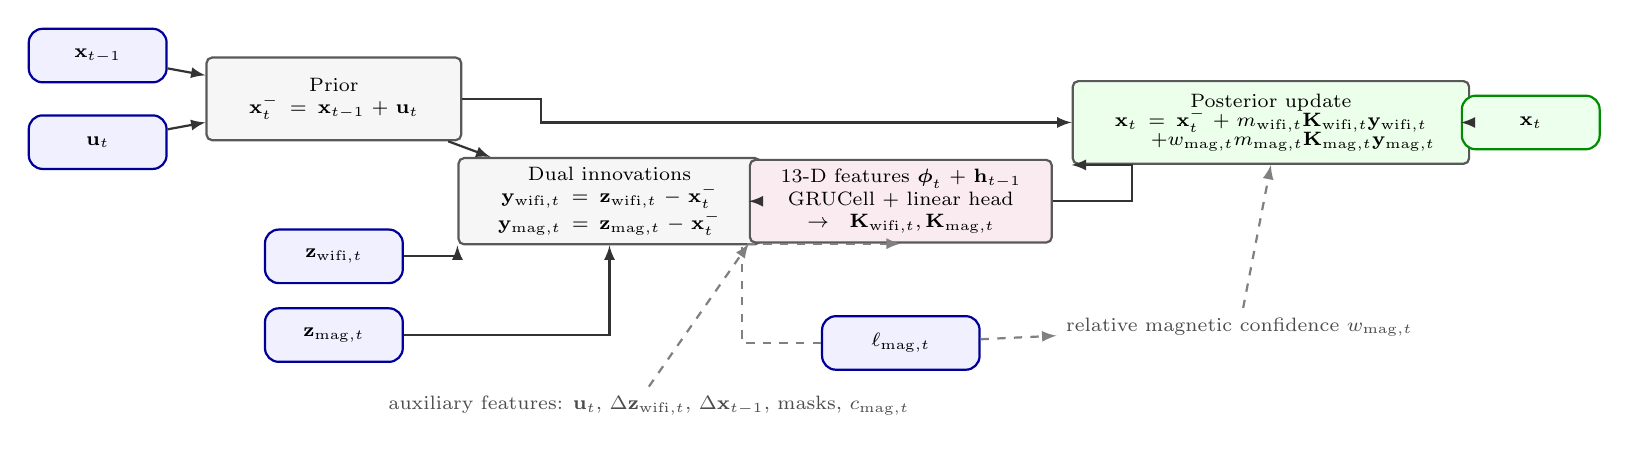
\begin{tikzpicture}[
    sig/.style={rectangle, rounded corners=5pt, draw=blue!60!black, thick, fill=blue!6,
        minimum height=0.68cm, minimum width=1.75cm, text centered, font=\scriptsize},
    blk/.style={rectangle, rounded corners=2pt, draw=black!65, thick, fill=gray!7,
        minimum height=1.05cm, text width=3.0cm, text centered, font=\scriptsize},
    learned/.style={blk, fill=purple!8, text width=3.6cm},
    update/.style={blk, fill=green!8, text width=4.8cm},
    line/.style={draw, -latex, thick, black!80},
    aux/.style={draw, -latex, dashed, thick, black!50},
    note/.style={font=\scriptsize, text=black!70, align=center}
]
    \node[sig] (xprev) at (0,2.0) {$\mathbf{x}_{t-1}$};
    \node[sig] (motion) at (0,0.9) {$\mathbf{u}_t$};
    \node[blk] (prior) at (3.0,1.45) {Prior\\$\mathbf{x}_t^-=\mathbf{x}_{t-1}+\mathbf{u}_t$};

    \node[sig] (wifi) at (3.0,-0.55) {$\mathbf{z}_{\mathrm{wifi},t}$};
    \node[sig] (mag) at (3.0,-1.55) {$\mathbf{z}_{\mathrm{mag},t}$};
    \node[blk, text width=3.6cm] (innov) at (6.5,0.15) {Dual innovations\\
        $\mathbf{y}_{\mathrm{wifi},t}=\mathbf{z}_{\mathrm{wifi},t}-\mathbf{x}_t^-$\\
        $\mathbf{y}_{\mathrm{mag},t}=\mathbf{z}_{\mathrm{mag},t}-\mathbf{x}_t^-$};

    \node[learned] (gru) at (10.2,0.15) {13-D features $\boldsymbol{\phi}_t$ + $\mathbf{h}_{t-1}$\\
        GRUCell + linear head\\
        $\to\ \mathbf{K}_{\mathrm{wifi},t},\mathbf{K}_{\mathrm{mag},t}$};

    \node[update] (post) at (14.9,1.15) {Posterior update\\[-1pt]
        $\mathbf{x}_t=\mathbf{x}_t^-+m_{\mathrm{wifi},t}\mathbf{K}_{\mathrm{wifi},t}\mathbf{y}_{\mathrm{wifi},t}$\\[-1pt]
        $\qquad +w_{\mathrm{mag},t}m_{\mathrm{mag},t}\mathbf{K}_{\mathrm{mag},t}\mathbf{y}_{\mathrm{mag},t}$};
    \node[sig, draw=green!55!black, fill=green!7] (out) at (18.2,1.15) {$\mathbf{x}_t$};

    \node[sig, minimum width=2.0cm] (ell) at (10.2,-1.65) {$\ell_{\mathrm{mag},t}$};
    \node[note] (weight) at (14.5,-1.45) {relative magnetic confidence $w_{\mathrm{mag},t}$};
    \node[note] (auxnote) at (7.0,-2.45) {auxiliary features: $\mathbf{u}_t$, $\Delta\mathbf{z}_{\mathrm{wifi},t}$, $\Delta\mathbf{x}_{t-1}$, masks, $c_{\mathrm{mag},t}$};

    \path[line] (xprev) -- (prior);
    \path[line] (motion) -- (prior);
    \path[line] (prior) -- (innov);
    \path[line] (wifi) -| (innov.south west);
    \path[line] (mag) -| (innov.south);
    \path[line] (innov) -- (gru);
    \path[line] (prior.east) -- ++(1.0,0) |- (post.west);
    \path[line] (gru.east) -- ++(1.0,0) |- (post.south west);
    \path[line] (post) -- (out);

    \path[aux] (ell) -- (weight);
    \path[aux] (weight) -- (post.south);
    \path[aux] (ell.west) -- ++(-1.0,0) |- (gru.south);
    \path[aux] (auxnote.north) -- (gru.south west);
\end{tikzpicture}
}
\caption{One DualKalmanNet update. PDR propagates the prior state, Wi-Fi and magnetic fixes form separate Cartesian innovations, and a recurrent gain predictor produces one $2\times2$ gain per modality. The posterior applies availability masks and the relative magnetic-confidence weight before producing $\mathbf{x}_t$. The remaining recurrent features are listed explicitly in the text below.}
\label{fig:arch_diagram}
\end{figure*}

\subsection{Wi-Fi Heatmap Measurement Model}\label{sec:wifi_model}

The MLP maps the normalized scan $\tilde{\mathbf{s}}_t$ to logits over the $M$ grid cells and then applies softmax, producing $\mathbf{p}_t\in[0,1]^M$ with
\begin{equation}
p_{t,c}\ge 0,\qquad \sum_{c=1}^{M}p_{t,c}=1.
\label{eq:softmax_def}
\end{equation}
Here $p_{t,c}$ is the learned probability mass assigned to grid cell $c$ at fusion step $t$.
\begin{figure*}[htbp]
\centering
\resizebox{0.99\textwidth}{!}{
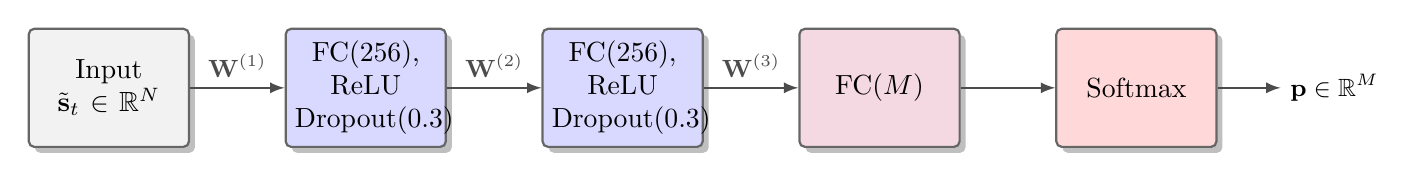
\begin{tikzpicture}[
    layer/.style={rectangle, draw=black!60, thick, fill=blue!10, text centered, rounded corners=2pt, minimum height=1.5cm, drop shadow, text width=1.8cm},
    arrow/.style={draw, thick, -latex, color=black!70},
    label/.style={font=\small\sffamily}
]
    % Nodes (Horizontal layout)
    \node[layer, fill=gray!10] (input) {Input\\$\tilde{\mathbf{s}}_t \in \mathbb{R}^N$};

    \node[layer, right=1.2cm of input, fill=blue!15] (fc1) {FC(256), ReLU\\Dropout(0.3)};
    \node[layer, right=1.2cm of fc1, fill=blue!15] (fc2) {FC(256), ReLU\\Dropout(0.3)};
    \node[layer, right=1.2cm of fc2, fill=purple!15] (fc3) {FC($M$)};

    \node[layer, right=1.2cm of fc3, fill=red!15] (softmax) {Softmax};
    \node[label, right=0.8cm of softmax] (output) {$\mathbf{p} \in \mathbb{R}^M$};

    % Arrows
    \path [arrow] (input) -- (fc1) node[midway, above, label] {$\mathbf{W}^{(1)}$};
    \path [arrow] (fc1) -- (fc2) node[midway, above, label] {$\mathbf{W}^{(2)}$};
    \path [arrow] (fc2) -- (fc3) node[midway, above, label] {$\mathbf{W}^{(3)}$};
    \path [arrow] (fc3) -- (softmax);
    \path [arrow] (softmax) -- (output);
\end{tikzpicture}
}
\caption{Architecture of the Wi-Fi multilayer perceptron (MLP) environment model. Dense layers sequentially extract features from the RSSI vector to compute an $M$-dimensional probability heatmap.}
\label{fig:mlp_arch}
\end{figure*}

At inference, the Cartesian Wi-Fi measurement is the softmax expectation
\begin{equation}
\mathbf{z}_{\mathrm{wifi},t}=\sum_{c=1}^{M}p_{t,c}\mathbf{c}_c,
\label{eq:heatmap_centroid}
\end{equation}
where $\mathbf{c}_c\in\mathbb{R}^2$ is the physical coordinate of grid cell $c$. DualKalmanNet consumes $\mathbf{z}_{\mathrm{wifi},t}$ directly; a heatmap covariance is not part of its 13-dimensional GRU input. Thus, the Wi-Fi branch supplies an intermittent absolute Cartesian anchor to the fusion stage.

\subsection{Magnetic Sequence Measurement Model}\label{sec:mag_model}

The magnetic branch complements the Wi-Fi anchor with a causal sequence-based spatial measurement. Let $n_t$ denote the raw-sample index at the end of fusion step $t$. The magnetic input is the causal feature window
\begin{equation}
\mathbf{M}_t=
\begin{bmatrix}
(\mathbf{f}^{\mathrm{mag}}_{n_t-T+1})^T\\
\vdots\\
(\mathbf{f}^{\mathrm{mag}}_{n_t})^T
\end{bmatrix}
\in\mathbb{R}^{T\times4},\qquad T=84.
\label{eq:mag_window}
\end{equation}
No future raw sample is included. The CNN maps $\mathbf{M}_t$ to the Cartesian measurement $\mathbf{z}_{\mathrm{mag},t}\in\mathbb{R}^2$ and scalar log-uncertainty score $\ell_{\mathrm{mag},t}\in\mathbb{R}$.

\begin{figure*}[htbp]
\centering
\resizebox{0.99\textwidth}{!}{
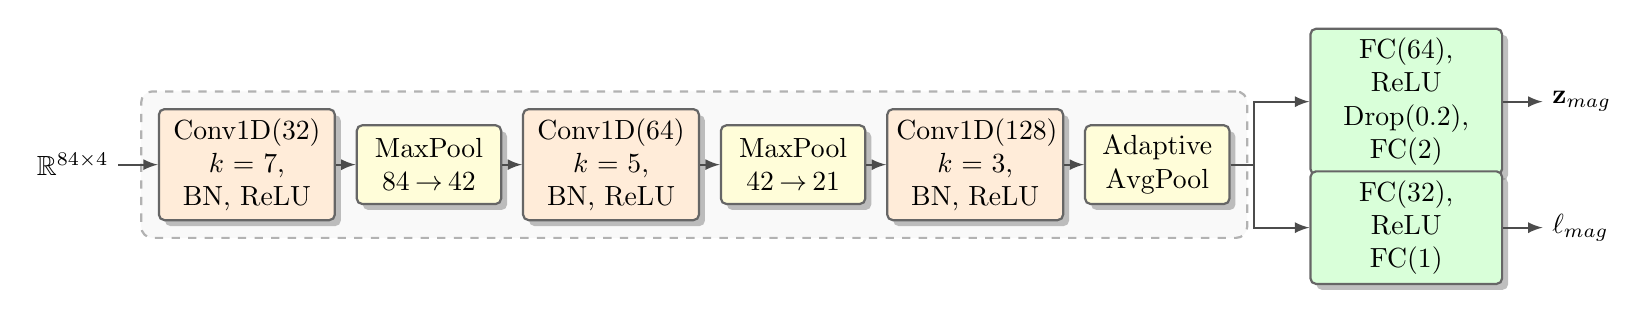
\begin{tikzpicture}[
    conv/.style={rectangle, draw=black!60, thick, fill=orange!15, text centered, rounded corners=2pt, minimum height=1cm, drop shadow, text width=2cm},
    pool/.style={rectangle, draw=black!60, thick, fill=yellow!15, text centered, rounded corners=2pt, minimum height=1cm, drop shadow, text width=1.6cm},
    head/.style={rectangle, draw=black!60, thick, fill=green!15, text centered, rounded corners=2pt, minimum height=1cm, drop shadow, text width=2.2cm},
    arrow/.style={draw, thick, -latex, color=black!70},
    groupbox/.style={rectangle, draw=black!30, dashed, thick, inner sep=6pt, rounded corners}
]
    \node (input) {$\mathbb{R}^{84 \times 4}$};
    \node[conv, right=0.5cm of input] (conv1) {Conv1D(32)\\$k\!=\!7$, BN, ReLU};
    \node[pool, right=0.25cm of conv1] (pool1) {MaxPool\\$84\!\to\!42$};
    \node[conv, right=0.25cm of pool1] (conv2) {Conv1D(64)\\$k\!=\!5$, BN, ReLU};
    \node[pool, right=0.25cm of conv2] (pool2) {MaxPool\\$42\!\to\!21$};
    \node[conv, right=0.25cm of pool2] (conv3) {Conv1D(128)\\$k\!=\!3$, BN, ReLU};
    \node[pool, right=0.25cm of conv3] (gap) {Adaptive\\AvgPool};
    \begin{scope}[on background layer]
        \node[groupbox, fill=gray!5, fit=(conv1) (gap)] (encoder_box) {};
    \end{scope}
    \node[head, right=1cm of gap, yshift=0.8cm] (pos_head) {FC(64), ReLU\\Drop(0.2), FC(2)};
    \node[head, right=1cm of gap, yshift=-0.8cm] (unc_head) {FC(32), ReLU\\FC(1)};
    \node[right=0.5cm of pos_head] (outpos) {$\mathbf{z}_{mag}$};
    \node[right=0.5cm of unc_head] (outunc) {$\ell_{mag}$};
    \path [arrow] (input) -- (conv1);
    \path [arrow] (conv1) -- (pool1);
    \path [arrow] (pool1) -- (conv2);
    \path [arrow] (conv2) -- (pool2);
    \path [arrow] (pool2) -- (conv3);
    \path [arrow] (conv3) -- (gap);
    \draw [arrow] (gap.east) -- ++(0.3,0) |- (pos_head.west);
    \draw [arrow] (gap.east) -- ++(0.3,0) |- (unc_head.west);
    \path [arrow] (pos_head) -- (outpos);
    \path [arrow] (unc_head) -- (outunc);
\end{tikzpicture}
}
\caption{Code-accurate architecture of the magnetic sequence CNN for $T=84$. The shared Conv1D encoder reduces the temporal length $84\to42\to21$ before adaptive global averaging into a 128-dimensional representation. Separate heads predict the 2-D magnetic position fix $\mathbf{z}_{\mathrm{mag}}$ and a scalar log-uncertainty score $\ell_{\mathrm{mag}}$.}
\label{fig:cnn_arch}
\end{figure*}

For $T=84$, the encoder maps $[B,4,84]$ to $[B,32,84]$, $[B,32,42]$, $[B,64,42]$, $[B,64,21]$, and finally $[B,128,21]$. Adaptive average pooling aggregates all 21 temporal locations into a shared $128$-dimensional vector. The position head is $128\!\to\!64\!\to\!2$ with ReLU and dropout $p=0.2$, while the scalar uncertainty head is $128\!\to\!32\!\to\!1$ with ReLU in its hidden layer. Thus the second output is learned from the same complete 84-frame representation as the position estimate; it is not computed analytically from the position residual at inference time.

$\ell_{\mathrm{mag},t}$ is used only as a relative uncertainty indicator; its training objective is given in Section~\ref{sec:setup}. Together, the Wi-Fi and magnetic branches provide the absolute spatial measurements used for correction; PDR supplies the relative motion used between those measurements.

\subsection{Causal PDR Motion Model}\label{sec:pdr}

PDR complements the learned absolute measurements by propagating relative motion between their updates~\cite{nnwifipdr,axesmapping}. At raw sampling rate $f_s=16.7$~Hz, an exponential moving average provides the baseline used by the causal threshold detector,
\begin{equation}
\bar{a}_n = \alpha\bar{a}_{n-1} + (1-\alpha)a_n,
\qquad \alpha=0.98,
\label{eq:lpf}
\end{equation}
with $\bar{a}_0=9.81$~m/s$^2$, and
\begin{equation}
\tilde{a}_n=a_n-\bar{a}_n.
\label{eq:hpf}
\end{equation}
Let $n_{\mathrm{last}}$ be the raw index of the most recently detected step. The binary step indicator is
\begin{equation}
d_n=\mathbb{1}\!\left[
\tilde{a}_n>\tau
\;\land\;
(n-n_{\mathrm{last}})>\Delta_r
\right],
\label{eq:step_trigger}
\end{equation}
where $\tau=0.6$~m/s$^2$ and $\Delta_r=\lfloor0.3f_s\rfloor=5$ frames; when $d_n=1$, the detector sets $n_{\mathrm{last}}\leftarrow n$. This detector uses only samples observed up to $n$.

The displacement contributed by raw sample $n$ is
\begin{equation}
\mathbf{v}_n=d_n L_s
\begin{bmatrix}
\cos\hat{\theta}_n\\
\sin\hat{\theta}_n
\end{bmatrix},
\qquad L_s=0.65~\mathrm{m}.
\label{eq:pdr_step}
\end{equation}
Let $\mathcal{B}_t$ denote the raw-sample indices assigned to fusion bin $t$. The PDR control consumed by DualKalmanNet is the accumulated bin displacement
\begin{equation}
\mathbf{u}_t=\sum_{n\in\mathcal{B}_t}\mathbf{v}_n
\in\mathbb{R}^2.
\label{eq:pdr}
\end{equation}
The evaluated estimator keeps $L_s$ fixed and treats $\hat{\theta}_n$ as an external causal heading observation; its synthetic noise model is specified in Section~\ref{sec:setup}. No ground-truth path length is used to adapt $L_s$.

\begin{figure}[htbp]
\centering
\resizebox{0.82\columnwidth}{!}{
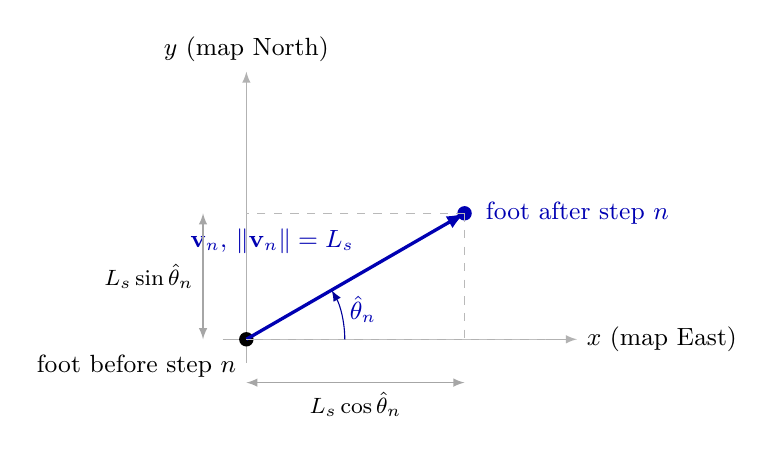
\begin{tikzpicture}[>=latex, thick, font=\small]
  \draw[->, gray!60, thin] (-0.3,0) -- (4.2,0) node[right, black] {$x$ (map East)};
  \draw[->, gray!60, thin] (0,-0.3) -- (0,3.4) node[above, black] {$y$ (map North)};
  \filldraw[black] (0,0) circle (2.2pt);
  \node[below left, yshift=-2pt] at (0,0) {foot before step $n$};
  \draw[->, very thick, blue!70!black] (0,0) -- ({3.2*0.866},{3.2*0.5})
        node[pos=0.56, above left=2pt, blue!70!black] {$\mathbf{v}_n$, $\|\mathbf{v}_n\|=L_s$};
  \filldraw[blue!70!black] ({3.2*0.866},{3.2*0.5}) circle (2.2pt);
  \node[right=4pt, blue!70!black] at ({3.2*0.866},{3.2*0.5}) {foot after step $n$};
  \draw[gray!50, dashed, thin] (0,0) -- (3.8,0);
  \draw[->, blue!60!black, thin] (1.25,0) arc[start angle=0, end angle=30, radius=1.25];
  \node[blue!70!black] at (1.48,0.38) {$\hat{\theta}_n$};
  \draw[gray!55, dashed, thin] ({3.2*0.866},{3.2*0.5}) -- ({3.2*0.866},0);
  \draw[<->, gray!70, thin] (0,-0.55) -- ({3.2*0.866},-0.55)
        node[midway, below, black, font=\footnotesize] {$L_s\cos\hat{\theta}_n$};
  \draw[gray!55, dashed, thin] ({3.2*0.866},{3.2*0.5}) -- (0,{3.2*0.5});
  \draw[<->, gray!70, thin] (-0.55,0) -- (-0.55,{3.2*0.5})
        node[midway, left, black, font=\footnotesize] {$L_s\sin\hat{\theta}_n$};
\end{tikzpicture}
}
\caption{Geometry of one detected PDR step. The per-sample displacement $\mathbf{v}_n$ has nominal length $L_s$ and is projected along the causal heading observation $\hat{\theta}_n$; fusion control $\mathbf{u}_t$ sums these step displacements over the raw samples in bin $t$.}
\label{fig:pdr_geometry}
\end{figure}

\subsection{Dual-Innovation KalmanNet Fusion}\label{sec:kalmannet}

The preceding modules provide PDR motion, Wi-Fi position, and magnetic position/confidence signals. DualKalmanNet combines these signals in a common Cartesian prediction/correction update. For an extended Kalman filter (EKF), after linearizing the measurement model with Jacobian $\mathbf{H}_t$, the analytical correction gain is
\begin{equation}
\mathbf{K}_t=\mathbf{P}_t^-\mathbf{H}_t^T
\left(\mathbf{H}_t\mathbf{P}_t^-\mathbf{H}_t^T+\mathbf{R}_t\right)^{-1},
\label{eq:ekf_gain}
\end{equation}
where $\mathbf{P}_t^-$ is the predicted state-error covariance and $\mathbf{R}_t$ is the assumed measurement-noise covariance. KalmanNet preserves a state-space prediction/correction structure but replaces this analytical gain computation with a recurrent learned mapping when parts of the dynamics or statistics are imperfectly known~\cite{kalmannet}. DualKalmanNet instead predicts separate gains for Wi-Fi and magnetic measurements. Using the bin-level PDR control from~(\ref{eq:pdr}), the prior state is
\begin{equation}
\mathbf{x}_{t}^{-}=\mathbf{x}_{t-1}+\mathbf{u}_t.
\label{eq:kn_predict}
\end{equation}
The two learned spatial measurements are expressed in the same Cartesian state space and produce
\begin{align}
\mathbf{y}_{\mathrm{wifi},t}
&=\mathbf{z}_{\mathrm{wifi},t}-\mathbf{x}_{t}^{-}
\in\mathbb{R}^{2},
\label{eq:kn_innovate_w}\\
\mathbf{y}_{\mathrm{mag},t}
&=\mathbf{z}_{\mathrm{mag},t}-\mathbf{x}_{t}^{-}
\in\mathbb{R}^{2}.
\label{eq:kn_innovate_m}
\end{align}
The pair $(\mathbf{y}_{\mathrm{wifi},t},\mathbf{y}_{\mathrm{mag},t})$ is the \emph{dual innovation}: two Cartesian measurement residuals formed against the same prior state.

The CNN additionally predicts $\ell_{\mathrm{mag},t}$ and the positive scale $q_{\mathrm{mag},t}=\exp(\ell_{\mathrm{mag},t})$. Because fusion uses only relative reliability, the reference score is computed from the fusion-training trajectories:
\begin{equation}
\begin{aligned}
\ell_{\mathrm{ref}}
&=\operatorname{median}_{(w,t)\in\mathcal{D}_{\mathrm{train}}:\,m_{\mathrm{mag},w,t}=1}
\ell_{\mathrm{mag},w,t},\\
q_{\mathrm{ref}}&=\exp(\ell_{\mathrm{ref}}),
\end{aligned}
\label{eq:mag_ref}
\end{equation}
where $w$ indexes a fusion-training walk. The relative magnetic confidence is
\begin{equation}
\begin{aligned}
w_{\mathrm{mag},t}
&=\frac{1}{1+\exp(r_t)},\\
r_t
&=\operatorname{clip}(\ell_{\mathrm{mag},t}-\ell_{\mathrm{ref}},-8,8),
\qquad 0<w_{\mathrm{mag},t}<1.
\end{aligned}
\label{eq:mag_weight}
\end{equation}
Thus scores above the training reference receive smaller explicit magnetic weights; clipping only limits the numerical range of the exponent. The same log-uncertainty score also enters the recurrent gain network as a separately clipped, masked feature.

For readability, the 13-dimensional recurrent input is listed explicitly below. Define
\begin{equation}
\begin{aligned}
\Delta\mathbf{x}_{t-1}&=\mathbf{x}_{t-1}-\mathbf{x}_{t-2},\\
c_{\mathrm{mag},t}&=m_{\mathrm{mag},t}\,
\operatorname{clip}(\ell_{\mathrm{mag},t},-6,8),
\end{aligned}
\label{eq:gru_aux}
\end{equation}
with $\Delta\mathbf{x}_{0}=\mathbf{0}$ at the first fusion update.
Then the input groups are
\begin{center}
\footnotesize
\begin{tabular}{@{}lc@{}}
\toprule
\textbf{GRU feature} & \textbf{Dim.} \\ \midrule
Masked Wi-Fi innovation $m_{\mathrm{wifi},t}\mathbf{y}_{\mathrm{wifi},t}$ & 2 \\
Masked magnetic innovation $m_{\mathrm{mag},t}\mathbf{y}_{\mathrm{mag},t}$ & 2 \\
Wi-Fi fix difference $\Delta\mathbf{z}_{\mathrm{wifi},t}$ & 2 \\
PDR control $\mathbf{u}_t$ & 2 \\
Previous posterior displacement $\Delta\mathbf{x}_{t-1}$ & 2 \\
Wi-Fi availability $m_{\mathrm{wifi},t}$ & 1 \\
Magnetic availability $m_{\mathrm{mag},t}$ & 1 \\
Magnetic confidence $c_{\mathrm{mag},t}$ & 1 \\ \midrule
\textbf{Total} & $\mathbf{13}$ \\ \bottomrule
\end{tabular}
\end{center}
Let
\begin{equation}
\kappa_t^{\mathrm{wifi}}
=\max\{k<t:\,m_{\mathrm{wifi},k}=1\}
\label{eq:wifi_previous_index}
\end{equation}
denote the previous fusion step with a Wi-Fi update, when such a step exists. The temporal Wi-Fi feature is
\begin{equation}
\Delta\mathbf{z}_{\mathrm{wifi},t}=
\begin{cases}
m_{\mathrm{wifi},t}
\left(\mathbf{z}_{\mathrm{wifi},t}-
\mathbf{z}_{\mathrm{wifi},\kappa_t^{\mathrm{wifi}}}\right),
& \kappa_t^{\mathrm{wifi}}\ \text{exists},\\
\mathbf{0}, & \text{otherwise}.
\end{cases}
\label{eq:wifi_delta}
\end{equation}
This is a short-term Wi-Fi consistency cue; it is zero when no new Wi-Fi fix is present. The eight feature groups in the table, concatenated in the displayed order, define $\boldsymbol{\phi}_t\in\mathbb{R}^{13}$. The recurrent gain generator implemented in code is
\begin{align}
\mathbf{h}_t
&=\operatorname{GRUCell}(\boldsymbol{\phi}_t,\mathbf{h}_{t-1})
\in\mathbb{R}^{64},
\label{eq:gru_recurrence}\\
\mathbf{g}_t
&=\mathbf{W}_K\mathbf{h}_t+\mathbf{b}_K
\in\mathbb{R}^{8},
\label{eq:gain_head}
\end{align}
with $\mathbf{h}_0=\mathbf{0}$. The first four components of $\mathbf{g}_t$ are reshaped into $\mathbf{K}_{\mathrm{wifi},t}\in\mathbb{R}^{2\times2}$ and the final four into $\mathbf{K}_{\mathrm{mag},t}\in\mathbb{R}^{2\times2}$.

Combining the prior in~(\ref{eq:kn_predict}), innovations in~(\ref{eq:kn_innovate_w})--(\ref{eq:kn_innovate_m}), learned gains, availability masks, and magnetic confidence in~(\ref{eq:mag_weight}) gives the posterior update
\begin{equation}
\mathbf{x}_t=\mathbf{x}_t^{-}
+m_{\mathrm{wifi},t}\mathbf{K}_{\mathrm{wifi},t}\mathbf{y}_{\mathrm{wifi},t}
+m_{\mathrm{mag},t}w_{\mathrm{mag},t}\mathbf{K}_{\mathrm{mag},t}\mathbf{y}_{\mathrm{mag},t}.
\label{eq:kn_correct}
\end{equation}
Setting an availability mask to zero removes that modality's correction. A large magnetic uncertainty score additionally reduces the magnetic term through $w_{\mathrm{mag},t}$. These equations define the causal inference update; the next section specifies how its measurement models and recurrent gain generator are trained and evaluated.

\section{Experimental Setup and Training}\label{sec:setup}

We evaluate the proposed fusion architecture in the IT Engineering building of the MagWi Benchmark Dataset~\cite{magwi}. Surveyed fingerprints define the environment resources used to generate Wi-Fi and magnetic measurements, while temporal fusion is evaluated on newly generated survey-graph-constrained trajectories. Consequently, the fusion experiment tests generalization to unseen trajectories within a fixed surveyed environment; it is not a held-out-device experiment. The magnetic evaluation also remains inside the per-phone-centered survey domain defined in Section~\ref{sec:measurements}; no online alignment of an uncalibrated handset to that domain is evaluated.

\subsection{Measurement-Model Training Objectives}

The Wi-Fi and magnetic measurement models are trained separately from temporal fusion.

\paragraph{Wi-Fi heatmap.}
For training example $i$, let $\mathbf{x}^{(i)}\in\mathbb{R}^2$ be the surveyed coordinate and $\mathbf{p}^{(i)}$ the MLP softmax output. The spatially graded target $\mathbf{q}^{(i)}\in\mathbb{R}^M$ is
\begin{equation}
q_c^{(i)}=
\frac{\exp\!\left(-\dfrac{\|\mathbf{c}_c-\mathbf{x}^{(i)}\|^2}{2\sigma^2}\right)}
{\displaystyle\sum_{r=1}^{M}\exp\!\left(-\dfrac{\|\mathbf{c}_r-\mathbf{x}^{(i)}\|^2}{2\sigma^2}\right)},
\qquad \sum_{c=1}^{M}q_c^{(i)}=1,
\label{eq:target_q}
\end{equation}
where $\sigma$ is the target spread. For a minibatch of size $B$, the implemented KL objective is
\begin{equation}
\mathcal{L}_{\mathrm{MLP}}
=\frac{1}{B}\sum_{i=1}^{B}\sum_{c=1}^{M}
q_c^{(i)}\log\!\left(\frac{q_c^{(i)}}{p_c^{(i)}}\right).
\label{eq:kl_loss}
\end{equation}

\paragraph{Magnetic sequence CNN.}
The CNN is trained on survey-derived, survey-graph-constrained magnetic sequences rather than directly on the raw MagWi continuous recordings. Random graph paths are sampled from the surveyed node proximity graph, interpolated at 16.7~Hz, and used to bilinearly sample the four-channel magnetic map; channel-wise Gaussian noise is added using the measured within-node variability.

Each generated 84-frame window uses the Cartesian position at its final frame as the regression target.

Let $\ell_{\mathrm{mag}}^{(i)}$ denote the scalar score for training window $i$ and define $q_{\mathrm{mag}}^{(i)}=\exp(\ell_{\mathrm{mag}}^{(i)})$. The implemented training objective is the uncertainty-weighted regression objective
\begin{equation}
\mathcal{L}_{CNN}=\frac{1}{B}\sum_{i=1}^{B}\left[
\frac{\|\mathbf{z}_{\mathrm{mag}}^{(i)}-\mathbf{x}_{\mathrm{true}}^{(i)}\|^2}{2\,\tilde q_{\mathrm{mag}}^{(i)}}
+\frac{1}{2}\ell_{\mathrm{mag}}^{(i)}\right],
\label{eq:nll_loss}
\end{equation}
where $\tilde q_{\mathrm{mag}}^{(i)}=\max(q_{\mathrm{mag}}^{(i)},0.01)$. A difficult sample can therefore receive a larger learned scale, reducing the first term, while the positive log-scale penalty discourages arbitrarily large uncertainty scores.

Importantly, (\ref{eq:nll_loss}) is \emph{not} the exact negative log-likelihood of a two-dimensional isotropic Gaussian: for a covariance $q\mathbf{I}_2$, the Gaussian normalization contributes $\log q$, rather than $\tfrac{1}{2}\log q$. We therefore do not interpret $q_{\mathrm{mag}}$ as a calibrated Cartesian variance or covariance. It is used only as a learned relative uncertainty/difficulty scale; the fusion stage consumes only its training-normalized relative value.

\subsection{Survey-Derived Synthetic Trajectory Evaluation}

The final fusion benchmark is synthetic because the continuous MagWi recordings do not provide the per-frame trajectory ground truth required for supervised KalmanNet training and controlled temporal evaluation. The simulator has access to the generated ground-truth state in order to produce sensor observations; the estimator does not. Specifically:

\begin{itemize}
    \item \textbf{Survey environment:} A Euclidean $\varepsilon$-proximity graph ($\varepsilon=1.6$~m) is built from surveyed IT Engineering reference-node coordinates. It uses no wall or obstacle geometry. The processed survey database is also used to construct a pool of real Wi-Fi scans and an interpolated four-channel magnetic map after per-phone centering. These environment resources include the available surveyed devices, and the simulator samples directly from the centered magnetic domain; therefore the fusion results are not claimed as an unseen-device test or as validation of causal handset-to-map alignment.
    \item \textbf{Trajectory generation:} Random endpoint pairs are sampled on the connected survey-node proximity graph and joined by shortest paths. Each path is interpolated at $16.7$~Hz with walking speed sampled uniformly from $1.0$ to $1.35$~m/s. Fusion training uses seed 1. Seed 2 is retained as the development protocol used before the final freeze, while the untouched final-test trajectories are generated with seed 4 only after the architecture, preprocessing, and metrics are fixed. The implementation hashes the resulting binned target trajectories and aborts if an identical training/final-test trajectory occurs in both sets.
    \item \textbf{Estimator initialization:} For each generated walk, the starting coordinate $\mathbf{x}_{\mathrm{start}}$ is subtracted from the Wi-Fi fixes, magnetic fixes, and target trajectory before KalmanNet training/evaluation. The recurrent estimator therefore starts from $\mathbf{x}_0=\mathbf{0}$ in translated coordinates, which is equivalent to assuming that the initial 2-D position is known. No subsequent ground-truth state is supplied as an estimator input.
    \item \textbf{PDR measurements:} At raw sample $n$, the simulator computes $\theta^{\mathrm{true}}_n$ from the displacement between the current and previous simulated positions only, then forms
    \begin{equation}
    \hat{\theta}_n=\theta^{\mathrm{true}}_n+b_n+\epsilon_n,
    \label{eq:sim_heading}
    \end{equation}
    where $b_n$ is a Gaussian random walk with per-frame standard deviation $0.5^{\circ}/\sqrt{16.7}$ and $\epsilon_n$ is zero-mean white noise with standard deviation $8.8^{\circ}$. Acceleration magnitude is synthesized as a step-frequency sinusoid (frequency sampled from 1.7--2.0~Hz) around gravity with additive Gaussian noise, then passed through the causal step detector of Section~\ref{sec:pdr}. Raw step displacements are summed within each of the 160 fusion bins according to~(\ref{eq:pdr}).
    \item \textbf{Wi-Fi measurements:} At each scheduled scan time, the nearest surveyed node to the true simulated position is located, one stored RSSI fingerprint from that node is sampled, and the trained Wi-Fi heatmap network produces $\mathbf{z}_{\mathrm{wifi},t}$. The degraded regime changes the scan interval to 5~s and independently drops 40\% of AP entries before inference.
    \item \textbf{Magnetic measurements:} The four rotation-invariant magnetic channels are bilinearly sampled from the survey-derived magnetic map along the simulated path, perturbed using the measured map-noise scale, and passed through the trained 84-frame magnetic CNN. Only causal windows ending at the current fusion time produce $\mathbf{z}_{\mathrm{mag},t}$ and $\ell_{\mathrm{mag},t}$.
    \item \textbf{Estimator/ground-truth separation:} KalmanNet receives only binned PDR controls, Wi-Fi fixes and masks, magnetic CNN fixes and masks, and magnetic log-uncertainty score. The generated ground-truth positions are used only to construct the simulated sensor observations and as the supervised training/evaluation target; they are never included in the KalmanNet input vector.
\end{itemize}

We generate 250 fusion-training trajectories and 60 untouched final-test trajectories, each represented by 160 fusion bins. The final test set is evaluated only after the method and metric definitions are frozen. This protocol provides controlled temporal ground truth while preserving a strict separation between the simulator's latent state and the observations supplied to the estimator. Mean errors and 95\% confidence-interval half-widths are computed from the 60 per-trajectory mean errors, with half-width $1.96$ times their standard error for one fixed trained model; retraining variability is not included. Median, P90, maximum, and CDF statistics use all $60\times160=9600$ pointwise localization errors.

\subsection{Training Details}

All neural components are implemented in PyTorch. The Wi-Fi MLP is optimized with Adam ($\beta_1=0.9$, $\beta_2=0.999$, weight decay $10^{-4}$) at a fixed learning rate of $10^{-3}$. The magnetic CNN uses the same Adam settings together with a ReduceLROnPlateau scheduler (patience 8, factor 0.5). The MLP uses dropout $p=0.3$ and a Gaussian target with spatial standard deviation $\sigma=2.0$~m. The MLP is trained for 80 epochs and the CNN for 60 epochs. The 1-D CNN magnetic sequence matcher uses $T=84$ frames (5.0~s at 16.7~Hz), selected from the candidate set $\{50,84,134,167\}$ on a 60-trajectory development set generated with seed 200. No standalone magnetic final-test number is reported. The KalmanNet GRU is trained for 150 epochs with Adam, learning rate $2\times10^{-3}$, weight decay $10^{-5}$, and mean squared error against ground-truth trajectories. For each signal-availability regime, the reference magnetic log-uncertainty score $\ell_{\mathrm{ref}}$ in~(\ref{eq:mag_ref}) is computed only from the 250 fusion-training trajectories and then frozen for evaluation.

The final fusion benchmark uses survey-derived environment resources from the available processed fingerprints and therefore is not a held-out-device experiment. Its errors measure generalization to untouched synthetic trajectories within the surveyed IT Engineering environment. In particular, the magnetic fusion pipeline assumes the survey-centered feature domain and does not evaluate causal normalization of a new handset.

\section{Experimental Results}\label{sec:results}

\subsection{Final Untouched-Trajectory Comparison}

Table~\ref{tab:fusion_comparison} reports the frozen seed-4 final-test results under full and degraded Wi-Fi. The non-temporal KNN baseline uses contemporaneous Wi-Fi and magnetic CNN measurements, magnetic log-uncertainty, and availability masks, but no PDR or recurrent history. Its $K$ is selected by five-fold grouped cross-validation on the training trajectories only ($K=5$ for full Wi-Fi and $K=20$ for degraded Wi-Fi).

\begin{table}[htbp]
\caption{Final Comparison on 60 Untouched Seed-4 Trajectories}
\label{tab:fusion_comparison}
\centering
\footnotesize
\setlength{\tabcolsep}{1.5pt}
\renewcommand{\arraystretch}{1.08}
\begin{tabular}{@{}p{0.16\columnwidth}p{0.32\columnwidth}p{0.23\columnwidth}p{0.12\columnwidth}p{0.12\columnwidth}@{}}
\toprule
\textbf{Regime} & \textbf{Model} & \textbf{Mean Err.} & \textbf{Med.} & \textbf{P90} \\ \midrule
Full Wi-Fi (1 Hz)
& Wi-Fi-only KalmanNet & 0.523 $\pm$ 0.052 m & 0.423 & 1.028 \\
& Wi-Fi+magnetic KNN & 0.745 $\pm$ 0.034 m & 0.510 & 1.613 \\
& \textbf{CNN Dual + rel. confidence} & \textbf{0.490 $\pm$ 0.046 m} & \textbf{0.403} & \textbf{0.976} \\ \midrule
Degraded Wi-Fi
& Wi-Fi-only KalmanNet & 1.734 $\pm$ 0.243 m & 1.243 & 3.767 \\
& Wi-Fi+magnetic KNN & 2.019 $\pm$ 0.187 m & 1.282 & 4.412 \\
& \textbf{CNN Dual + rel. confidence} & \textbf{0.900 $\pm$ 0.101 m} & \textbf{0.710} & \textbf{1.845} \\ \bottomrule
\end{tabular}
\end{table}

The weighted DualKalmanNet improves the final-test mean in both regimes. With full 1~Hz Wi-Fi, it reduces mean error by 6.4\% relative to Wi-Fi-only KalmanNet (0.523~m to 0.490~m) and reduces pointwise P90 from 1.028~m to 0.976~m. Under degraded Wi-Fi, the reduction is larger: mean error falls by 48.1\% (1.734~m to 0.900~m), while pointwise P90 falls from 3.767~m to 1.845~m. The non-temporal KNN baseline is worse than both temporal estimators in both regimes, supporting the value of PDR propagation and recurrent correction rather than simply exposing the same absolute measurements to a static regressor.

\begin{figure*}[t]
\centering
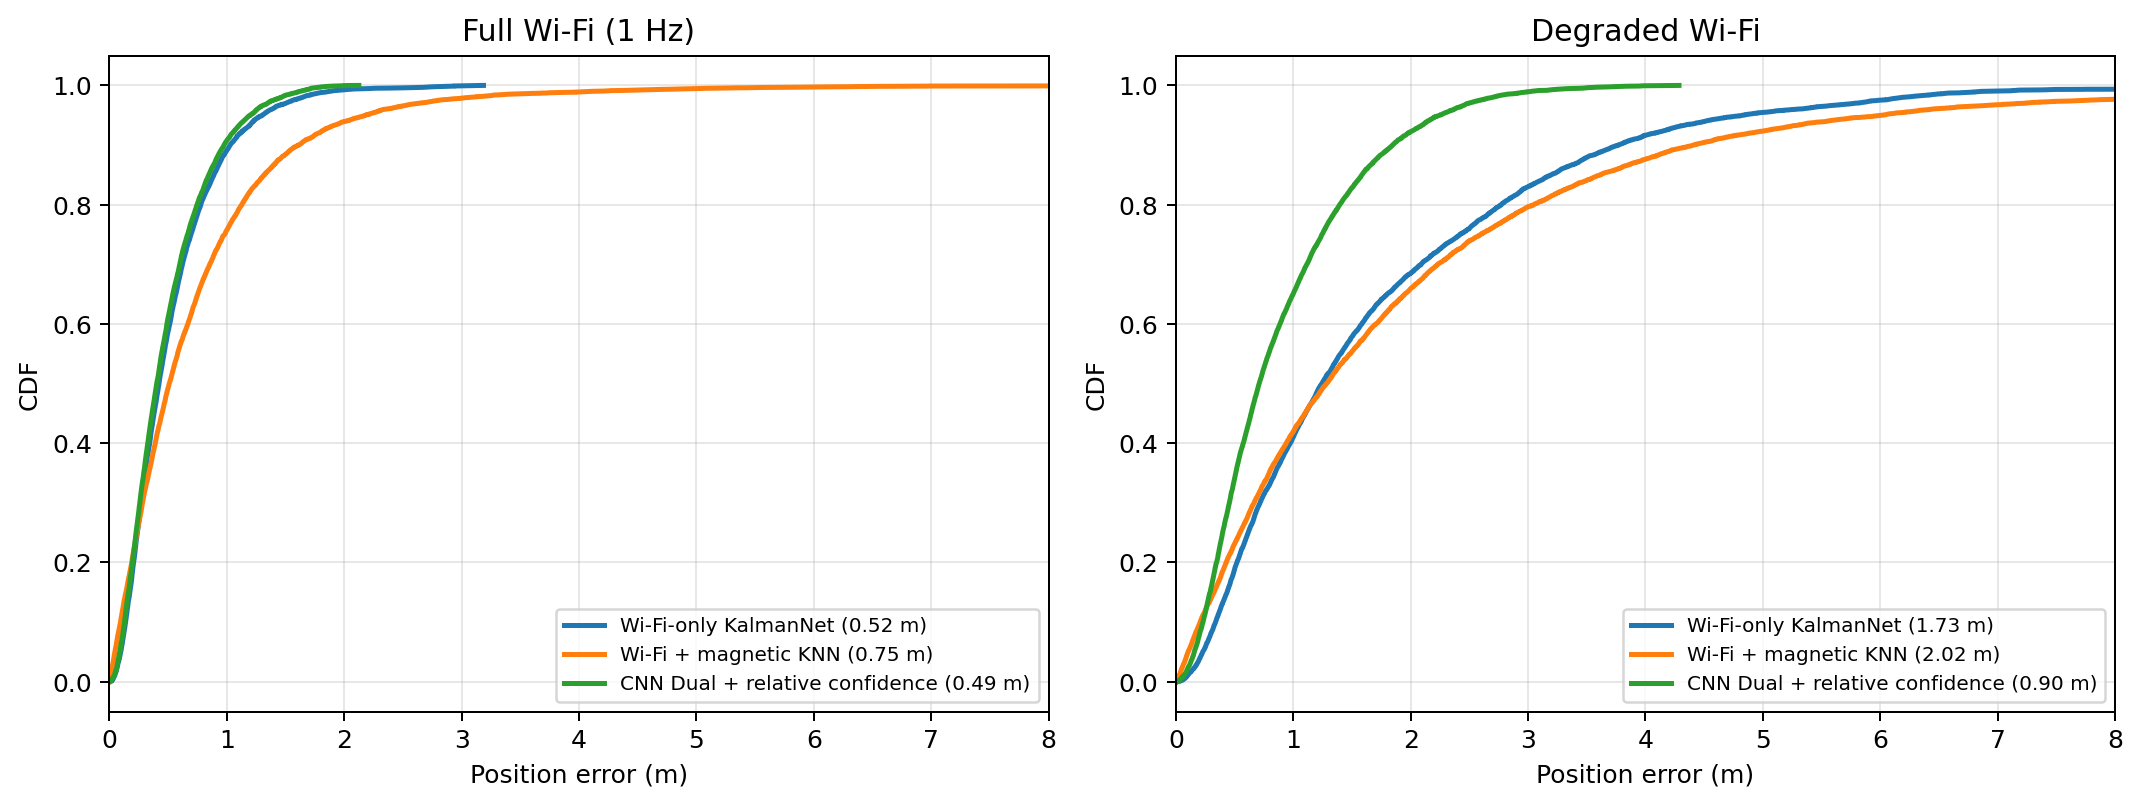
\includegraphics[width=0.92\textwidth]{../benchmarks/final_protocol/current_results/final_cdf.png}
\caption{Pointwise localization-error CDFs on the untouched seed-4 final set. Each panel contains all $60\times160=9600$ final-test points. The KNN baseline is non-temporal and uses no PDR or recurrent history. The horizontal axis is limited to 8~m for readability; the degraded-Wi-Fi KNN maximum is 27.95~m.}
\label{fig:final_cdfs}
\end{figure*}

Figure~\ref{fig:final_cdfs} shows the same comparison over all pointwise errors. In the full-Wi-Fi regime, the weighted model shifts the CDF modestly left of Wi-Fi-only KalmanNet. Under degraded Wi-Fi, the separation is substantially larger across the distribution and in the upper tail. These results are specific to the fixed surveyed environment and synthetic survey-graph trajectory protocol described above; they do not establish building-independent or unseen-device magnetic deployment.

\section{Conclusion}\label{sec:conclusion}

This paper presented a decoupled learned state-space architecture that separates spatial inference from temporal tracking. A Wi-Fi heatmap MLP and gravity-referenced magnetic sequence CNN provide Cartesian measurements, while DualKalmanNet predicts separate $2\!\times\!2$ gains; availability masks and relative magnetic uncertainty suppress missing or unreliable corrections. On the untouched final set, the weighted model reduces mean error from 0.523~m to 0.490~m with full Wi-Fi and from 1.734~m to 0.900~m under degraded Wi-Fi; in the degraded regime, pointwise P90 falls from 3.767~m to 1.845~m. The present results demonstrate trajectory generalization within one surveyed environment and require site-specific environment resources. They also assume access to the survey-centered magnetic feature domain; causal alignment of an uncalibrated handset to that domain is not evaluated. Future work will investigate such device-domain alignment without position ground truth and extend the state to three-dimensional multi-floor positioning with barometric altitude information.

\section*{Acknowledgment}
The authors acknowledge the Summer Undergraduate Research Award (SURA) program at the Indian Institute of Technology Delhi for supporting this research.

\bibliographystyle{ieeetr}
\bibliography{Ref}

\end{document}
